\documentclass[landscape,a0paper,fontscale=0.292]{baposter}

\usepackage[vlined]{algorithm2e}
\usepackage{times}
\usepackage{calc}
\usepackage{url}
\usepackage{graphicx}
\usepackage{amsmath}
\usepackage{amssymb}
\usepackage{relsize}
\usepackage{multirow}
\usepackage{booktabs}

\usepackage{graphicx}
\usepackage{multicol}
\usepackage[T1]{fontenc}
\usepackage{ae}
\usepackage{enumitem}
\usepackage[pagebackref=true,breaklinks=true,letterpaper=true,colorlinks,bookmarks=false,urlcolor  = blue,]{hyperref}
\usepackage{colortbl}
\usepackage{xcolor}
\graphicspath{{images/}}
\definecolor{salmon}{rgb}{1.0, 0.90, 0.75}
\definecolor{LightCyan}{rgb}{0.88,1,1}
\definecolor{azure}{rgb}{0.94, 1.0, 1.0}
\definecolor{khaki}{rgb}{0.94, 0.9, 0.55}
\definecolor{lemonchiffon}{rgb}{1.0, 0.98, 0.8}
\definecolor{mistyrose}{rgb}{1.0, 0.89, 0.88}
\definecolor{palerobineggblue}{rgb}{0.59, 0.87, 0.82}
\definecolor{mossgreen}{rgb}{0.68, 0.87, 0.68}
\definecolor{magicmint}{rgb}{0.77, 1, 0.92}
\definecolor{grannysmithapple}{rgb}{0.66, 0.89, 0.63}	\definecolor{lavenderblue}{rgb}{0.9, 0.9, 1.0}
\definecolor{peachorange}{rgb}{1.0, 0.8, 0.6}
\definecolor{pistachio}{rgb}{0.85, 1, 0.72}
\definecolor{brightmaroon}{rgb}{0.76, 0.13, 0.28}
\definecolor{bluencs}{rgb}{0.0, 0.53, 0.74}
\setlist[itemize]{leftmargin=*,nosep}
 \setlength{\columnsep}{0.7em}
 \setlength{\columnseprule}{0mm}


% %%%%%%%%%%%%%%%%%%%%%%%%%%%%%%%%%%%%%%%%%%%%%%%%%%%%%%%%%%%%%%%%%%%%%%%%%%%%%%%%
% % Save space in lists. Use this after the opening of the list
% %%%%%%%%%%%%%%%%%%%%%%%%%%%%%%%%%%%%%%%%%%%%%%%%%%%%%%%%%%%%%%%%%%%%%%%%%%%%%%%%
 \newcommand{\compresslist}{%
 \setlength{\itemsep}{0pt}%
 \setlength{\parskip}{0pt}%
 \setlength{\parsep}{0pt}%
 }
\renewcommand{\rmdefault}{ptm} % Arial
\renewcommand{\sfdefault}{ptm} % Arial

%%%%%%%%%%%%%%%%%%%%%%%%%%%%%%%%%%%%%%%%%%%%%%%%%%%%%%%%%%%%%%%%%%%%%%%%%%%%%
%% Begin of Document
%%%%%%%%%%%%%%%%%%%%%%%%%%%%%%%%%%%%%%%%%%%%%%%%%%%%%%%%%%%%%%%%%%%%%%%%%%%%%
\begin{document}
%%%%%%%%%%%%%%%%%%%%%%%%%%%%%%%%%%%%%%%%%%%%%%%%%%%%%%%%%%%%%%%%%%%%%%%%%%%%%
%% Here starts the poster
%%---------------------------------------------------------------------------
%% Format it to your taste with the options
%%%%%%%%%%%%%%%%%%%%%%%%%%%%%%%%%%%%%%%%%%%%%%%%%%%%%%%%%%%%%%%%%%%%%%%%%%%%%
\begin{poster}{
 % Show grid to help with alignment
 grid=false,
 columns=4,
 % Column spacing
 colspacing=0.7em,
 % Color style
 headerColorOne=cyan!20!white!90!black,
 borderColor=cyan!30!white!90!black,
 % Format of textbox
 textborder=faded,
 % Format of text header
 headerborder=open,
 headershape=roundedright,
 headershade=plain,
 background=none,
 bgColorOne=cyan!10!white,
 headerheight=0.12\textheight}
 % Eye Catcher
 {
      
\includegraphics[width=0.07\linewidth]{VGG_logo.jpg}
      \makebox[0.005\textwidth]{} 
      
\includegraphics[width=0.08\linewidth]{Google_Research.png}
      
    
 }
 % Title
 {\sc\huge\bf \textit{Speech2Action:} Cross-modal Supervision for Action Recognition}
 % Authors
 {Arsha Nagrani$^{1,2}$~~~~Chen Sun$^2$~~~~David Ross$^2$ ~~~~Rahul Sukthankar$^2$~~~~Cordelia Schmid$^{2}$ ~~~~Andrew Zisserman$^{1,3}$ \\[0.2em]

$^1$VGG, Oxford~~~~$^2$Google Research~~~~$^3$DeepMind~~~~  }
 {
  \begin{tabular}{r}
      %\makebox[0.01\textwidth]{} 
    
\includegraphics[width=0.12\linewidth]{CVPR_logo_2020.png}
  \end{tabular}
 }

%%%%%%%%%%%%%%%%%%%%%%%%%%%%%%%%%%%%%%%%%%%%%%%%%%%%%%%%%%%%%%%%%%%%%%%%%%%%%%
%%% Now define the boxes that make up the poster
%%%---------------------------------------------------------------------------
%%% Each box has a name and can be placed absolutely or relatively.
%%% The only inconvenience is that you can only specify a relative position 
%%% towards an already declared box. So if you have a box attached to the 
%%% bottom, one to the top and a third one which should be inbetween, you 
%%% have to specify the top and bottom boxes before you specify the middle 
%%% box.
%%%%%%%%%%%%%%%%%%%%%%%%%%%%%%%%%%%%%%%%%%%%%%%%%%%%%%%%%%%%%%%%%%%%%%%%%%%%%%

%%%%%%%%%%%%%%%%%%%%%%%%%%%%%%%%%%%%%%%%%%%%%%%%%%%%%%%%%%%%%%%%%%%%%%%%%%%%%%
\headerbox{\bf\color{blue} Problem Definition and Contribution}{name=contribution,column=0,row=0,span=1}{
   \textbf{\color{blue}Goal:} Action Recognition in Movies and TV shows using only the speech as supervision
  \begin{center}
   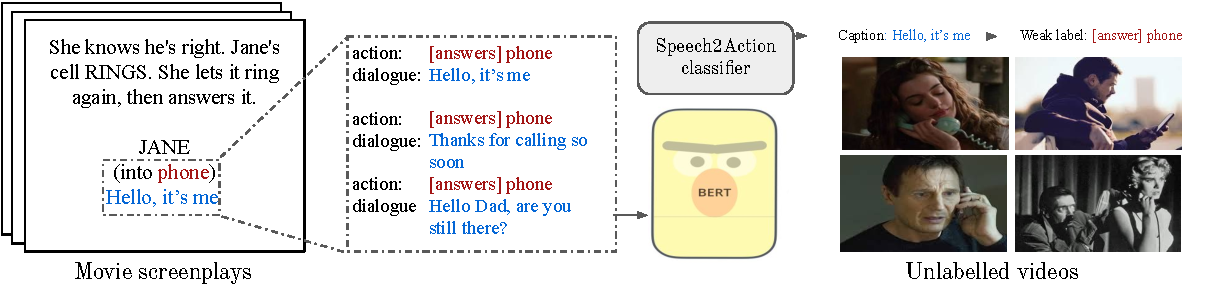
\includegraphics[width=1\textwidth]{images/teaser_6.pdf}
  \end{center}
    \textbf{\color{blue}Motivations:}
    \begin{itemize}
        \item Manual annotation of human actions is expensive and not scalable
        \item Videos accompanied by speech are available in large numbers online.
    \end{itemize}
    \textbf{\color{blue}Key Contributions:}
    \begin{itemize}
\item A \texttt{Speech2Action} model trained from literary screenplays that predicts actions from transcribed speech \textit{alone}  
\item By applying this \texttt{Speech2Action} model to a large unlabelled corpus of videos, we obtain obtain weak action labels for over 800K video clips 
\item Action classifier trained with these weak labels achieves state of the art results on HMDB51 
\item The action classifier with \textit{no} fine-tuning beats fully supervised performance on the AVA dataset. 
    \end{itemize}  
}

%%%%%%%%%%%%%%%%%%%%%%%%%%%%%%%%%%%%%%%%%%%%%%%%%%%%%%%%%%%%%%%%%%%%%%%%%%%%%
\headerbox{\bf\color{blue} IMSDb Dataset}{name=imsdb,column=1,row=0,span=1}{
% \begin{tabular}{c c c c c c c  } 
\toprule
\# movies &
\# scene descriptions &
\# speech segs &
\# sentences &
\# words &
\# unique words &
\# genres \\ 
 \midrule
1,070 &
539,827 &
595,227 &
2,570,993 &
21,364,357 &
590,959 &
22 \\ 
\bottomrule
\end{tabular}
\begin{itemize}
    \item Download 1,080 movie scripts from IMSDb.com spanning 22 genres 
    \item Separate out scene descriptions (which contain mention of \textbf{\textcolor{brightmaroon}{actions}}) and \textbf{\textcolor{bluencs}{speech segments}}. 
    \item Create a text dataset of \textbf{\textcolor{bluencs}{speech}} paired with \textbf{\textcolor{brightmaroon}{action}} labels, using proximity in the movie scripts as a cue.
\end{itemize}
        \begin{center}
            Examples of Movie Scripts 
       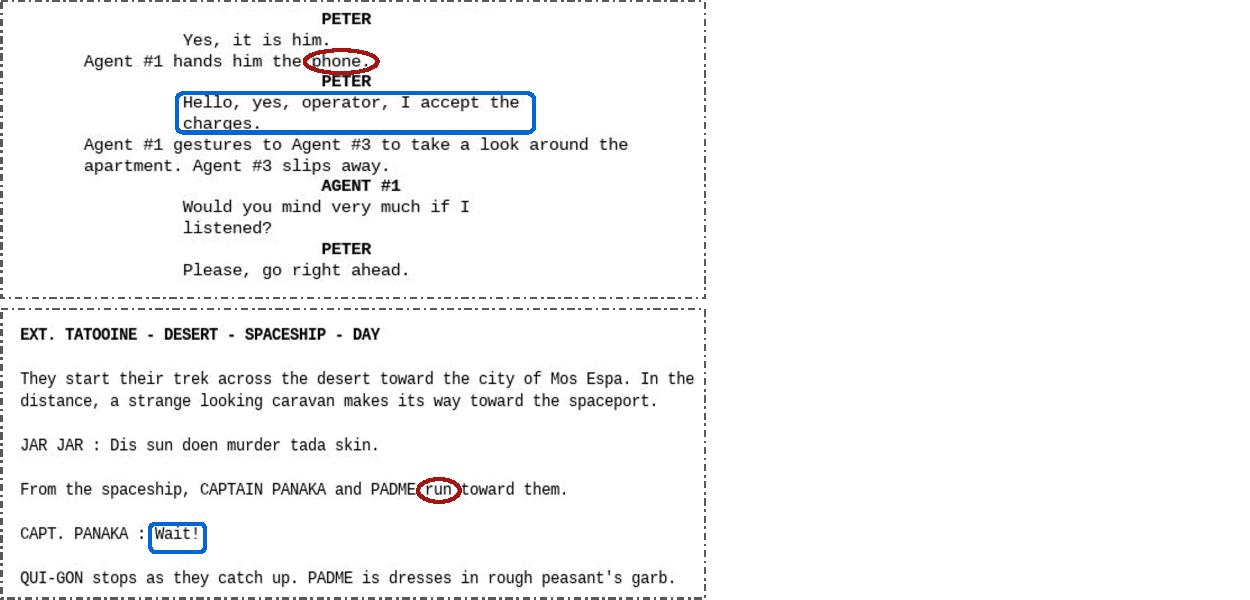
\includegraphics[width=\linewidth]{images/scripts_cropped.pdf}
        \end{center}
   
}

%%%%%%%%%%%%%%%%%%%%%%%%%%%%%%%%%%%%%%%%%%%%%%%%%%%%%%%%%%%%%%%%%%%%%%%%%%%%%
\headerbox{\bf\color{blue} Results on Visual Action Recognition}{name=results,column=2,row=0,span=2}{
    %     \begin{minipage}{0.93\textwidth}
    \resizebox{\textwidth}{!}{
    \Huge
        \begin{tabular}{c|*{4}{c}|*{4}{c}|*{4}{c}|*{4}{c}|*{4}{c}}
        \toprule
        \multirow{2}{*}{} & \multicolumn{4}{c}{Glass} 
                               & \multicolumn{4}{c}{Glass with Water} 
                               & \multicolumn{4}{c}{Lens} 
                               & \multicolumn{4}{c}{Complex Shape}  
                               & \multicolumn{4}{c}{Average}  \\
                               & \cellcolor{red!25} F-EPE & \cellcolor{red!25}A-MSE & \cellcolor{red!25}I-MSE & \cellcolor{blue!25} M-IoU 
                               & \cellcolor{red!25} F-EPE & \cellcolor{red!25}A-MSE & \cellcolor{red!25}I-MSE & \cellcolor{blue!25} M-IoU 
                               & \cellcolor{red!25} F-EPE & \cellcolor{red!25}A-MSE & \cellcolor{red!25}I-MSE & \cellcolor{blue!25} M-IoU 
                               & \cellcolor{red!25} F-EPE & \cellcolor{red!25}A-MSE & \cellcolor{red!25}I-MSE & \cellcolor{blue!25} M-IoU 
                               & \cellcolor{red!25} F-EPE & \cellcolor{red!25}A-MSE & \cellcolor{red!25}I-MSE & \cellcolor{blue!25} M-IoU \\
        \midrule
        Background    & 3.6 / 30.3 & 1.33 & 0.48 & 0.12 & 6.4 / 53.2 & 1.54 & 0.68 & 0.12 & 10.3 / 39.2 & 1.94 & 1.57 & 0.24 & 6.8 / 56.8 & 2.50 & 0.85 & 0.11 & 6.8 / 44.9 & 1.83 & 0.90 & 0.15 \\
        CoarseNet     & 2.1 / 15.8 & 0.22 & 0.14 & 0.97 & 3.1 / 23.5 & 0.31 & 0.23 & 0.97 & 2.0 / 6.7   & 0.17 & 0.28 & 0.99 & 4.5 / 34.4 & 0.38 & 0.33 & 0.92 & 2.9 / 20.1 & 0.27 & 0.24 & 0.96 \\
        \midrule
        TOM-Net       & 1.9 / 14.7 & 0.21 & 0.14 & 0.97 & 2.9 / 21.8 & 0.30 & 0.22 & 0.97 & 1.9 / 6.6   & 0.15 & 0.29 & 0.99 & 4.1 / 31.5 & 0.37 & 0.32 & 0.92 & 2.7 / 18.6 & 0.26 & 0.24 & 0.96 \\
        \bottomrule
    \end{tabular}
    }
    \end{minipage}
    \hspace{-0.6em}
    \begin{minipage}{0.06\textwidth}
        \resizebox{\textwidth}{!}{
        \begin{tabular}{cc}
            \midrule
            MSE ($\cdot10^{-2}$) \\
            \cellcolor{red!25} $\downarrow$ better \\ 
            \cellcolor{blue!25} $\uparrow$ better\\
            \midrule
        \end{tabular}
        }
    \end{minipage}



    \vspace{0.5em}
    \textbf{\color{blue}Examples of clips mined using Speech2Action:}
    \begin{center}
        \vspace{-0.8em}
        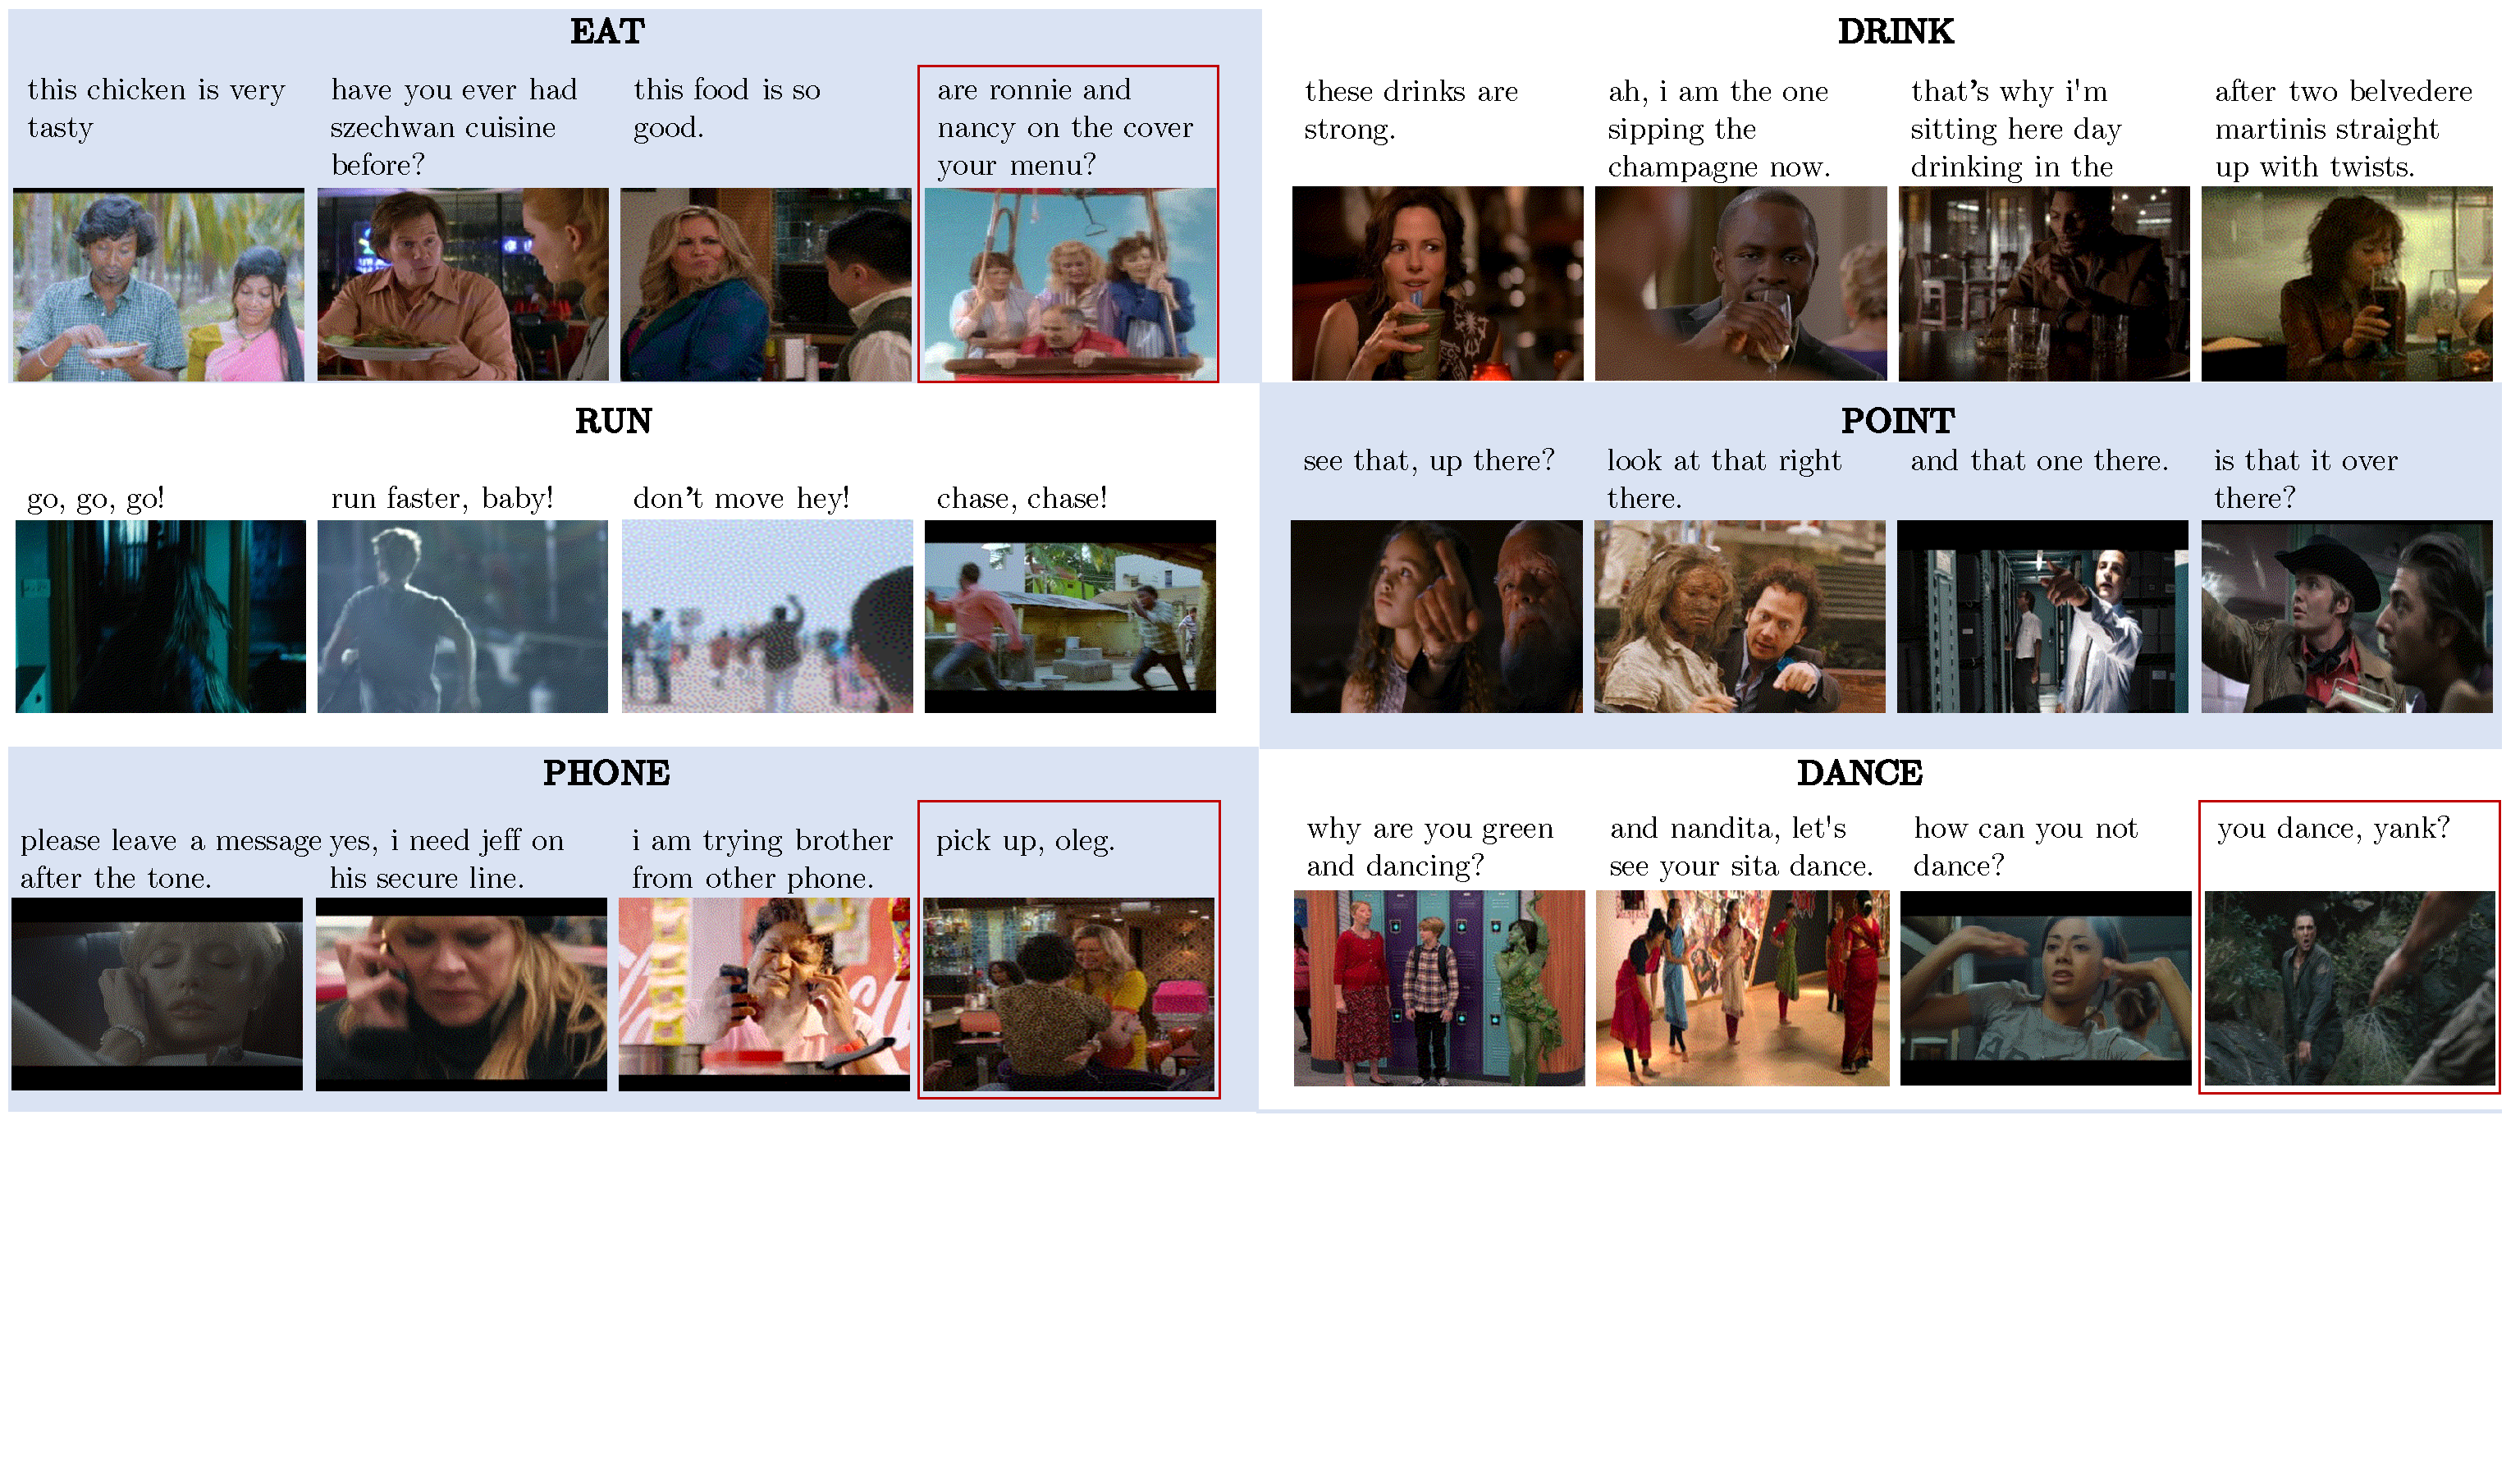
\includegraphics[width=0.9\linewidth]{images/mining_cropped.pdf}
        \vspace{-1em}
    \end{center}
\textbf{\color{blue}Examples of abstract actions mined using Speech2Action:}
    \begin{center}
     \vspace{-0.8em}
    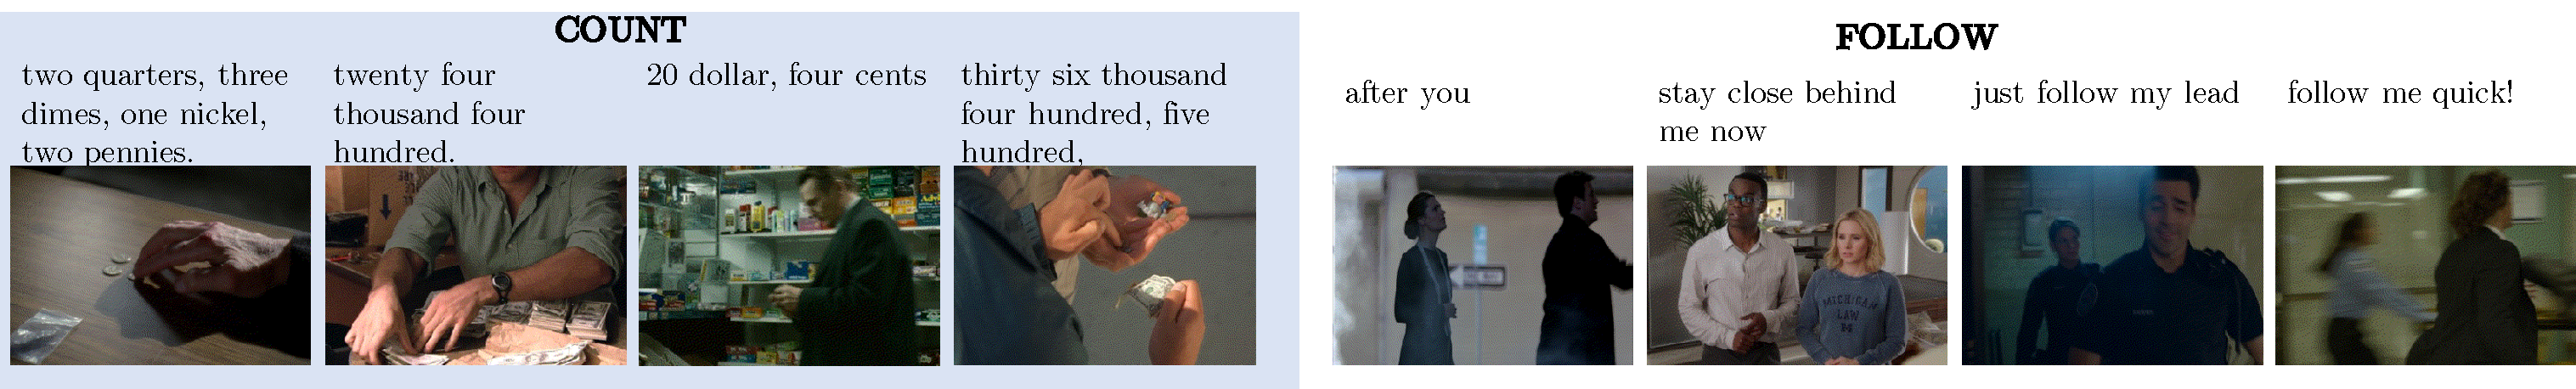
\includegraphics[width=0.92\linewidth]{images/mining_unusual.pdf}
    \vspace{-1em}
   \end{center}
    \vspace{0.5em}
    {\bf\color{blue}Results on 14 AVA mid and tail classes}
    \vspace{0.2em}
    
\centering 
\footnotesize{
\begin{tabular}{c c c c c c c c c c c c c c c c} 
\toprule
\multicolumn{1}{c}{\textbf{Data}}&
\multicolumn{14}{c}{\textbf{Per-Class AP}}  \\
% pre-training &
                              & drive & phone & kiss & dance & eat & drink & run & point & open & hit & shoot & push & hug & enter \\ 
\midrule
AVA \tiny{(fully supervised)} & 0.63  & 0.54  & 0.22 & 0.46  &0.67 & 0.27  & 0.66 & 0.02 & 0.49 & 0.62 & 0.08 & 0.09 & 0.29 &0.14 \\
\midrule
 \texttt{S2A-mined} \tiny{(zero-shot)} & \cellcolor{mistyrose}{0.83} & \cellcolor{mistyrose}{0.79} & 0.13 & \cellcolor{mistyrose}{0.55} & \cellcolor{mistyrose}{0.68} & \cellcolor{mistyrose}{0.30} & 0.63 &  \cellcolor{mistyrose}{0.04}& \cellcolor{mistyrose}{0.52} & 0.54 & \cellcolor{mistyrose}{0.18} & 0.04 & 0.07 & 0.04\\
\midrule
\texttt{S2A-mined} + AVA & \textbf{0.86} & \textbf{0.89} & \textbf{0.34} & \textbf{0.58} & \textbf{0.78} & \textbf{0.42} & \textbf{0.75} & 0.03 & \textbf{0.65} & \textbf{0.72} & \textbf{0.26} & \textbf{0.13} & \textbf{0.36} & \textbf{0.16}\\
% \midrule
% \texttt{S2A-mined } & AVA fewshot-10 & &  & &  & &  & & & &\\
% \texttt{S2A-mined } & AVA fewshot-50 & & & & & & & & & &\\
% \texttt{S2A-mined } & AVA fewshot-100 & & & & & & & & & &\\
% \texttt{S2A-mined } & AVA (all)       & & & & & & & & & &\\
 \bottomrule
\end{tabular}
}
\caption{{\textbf{Per-class average precision for $14$ AVA mid and tail classes.} These actions occur \textit{rarely}, and hence are harder to get manual supervision for. For 8 of the 14 classes, we exceed fully supervised performance without a single manually labelled training example. }}



% \begin{table*}[ht]
% \centering 
% \begin{tabular}{c c c c c c c c c c c c} 
% \toprule
% \multicolumn{2}{c}{\textbf{Data}}&
% \multicolumn{7}{c}{\textbf{Per-Class AP}}  \\
% pre-training & training &
% drive &
% phone &
% kiss &
% dance &
% eat &
% drink & run & point & open & hit\\ 
% \midrule
% \texttt{S2A-mined } & AVA fewshot-20 & 0.82 & 0.80 & 0.10 & 0.55 & 0.67 & 0.33 &  0.64& 0.04& 0.51 & 0.59\\
% \texttt{S2A-mined } & AVA fewshot-50 & 0.82 & 0.86 & 0.30 & 0.56 & 0.69 & 0.37 & 0.69& 0.05& 0.52 & 0.65\\
% \texttt{S2A-mined } & AVA fewshot-100 & & & & & & & & & &\\
% \texttt{S2A-mined } & AVA (all)       & & & & & & & & & &\\


% \bottomrule
% \end{tabular}
% \caption{Per-class average precision for $10$ AVA mid and tail classes using few-shot learning.}

    
\begin{minipage}{0.5\linewidth}
{\bf\color{blue}Action Recognition Model}
\begin{itemize}
    \item We train an S3D-G model for 18-way classification on video clips labelled with the Speech2Action model 
    \item We evaluate on AVA with NO finetuning, on mid and tail classes. These actions occur \textit{rarely}, and are hard to get manual supervision for. For 8 classes, we exceed fully supervised performance without a single manually labelled training example.
    \item On HMDB51, we obtain a 17\% improvement over training from scratch and also outperform previous self-supervised and weakly supervised works.
\end{itemize}
\end{minipage}   
\begin{minipage}{0.5\linewidth}
    \vspace{1em}
{\bf\color{blue} \quad Results on HMDB51}
\vspace{-0.3em}
\begin{flushright}

\centering 
\footnotesize{
\begin{tabular}{l l l l r}
\toprule
Method & Architecture  & Pre-training & Acc. \\
% Shuffle\&Learn (Misra {\it et al.}~\cite{misra2016shuffle}) & AlexNet~\cite{krizhevsky2012imagenet} & Scratch & 13.3 \\
% Shuffle\&Learn (Misra {\it et al.}~\cite{misra2016shuffle}) & AlexNet~\cite{krizhevsky2012imagenet} & Tuple verify~\cite{misra2016shuffle} &  18.1 \\
% Shuffle\&Learn (Misra {\it et al.}~\cite{misra2016shuffle}) & AlexNet~\cite{krizhevsky2012imagenet}  & ImageNet &  28.5 \\
% Two-stream (RGB)~\cite{simonyan2014two} & VGG-M~\cite{Simonyan_14a} & 1 & ImageNet & - & 40.5 \\
% C3D~\cite{carreira2017quo} & Custom  & Scratch & 24.3 & - \\
\arrayrulecolor{GrayLine}
% \midrule
% LSTM~\cite{carreira2017quo} & BN-Inception~\cite{ioffe2015batch} & - & ImageNet & 36.0 & - \\
% Two stream (RGB)~\cite{carreira2017quo} & BN-Inception~\cite{ioffe2015batch} & 1 & ImageNet & 43.2 & - \\
% I3D (RGB)~\cite{carreira2017quo} & BN-Inception~\cite{ioffe2015batch} & 64 & ImageNet & 49.8 & - \\
% \midrule

\midrule
Shuffle\&Learn & S3D-G (RGB) & UCF101& 35.8\\
OPN   & VGG-M-2048  & UCF101  & 23.8 \\
ClipOrder  & R(2+1)D  & UCF101   & 30.9 \\
3DRotNet & S3D-G (RGB)  & Kinetics   &  40.0 \\
DPC  & 3DResNet18 & Kinetics & 35.7 \\
CBT  & S3D-G (RGB) & Kinetics   & 44.6 \\
\midrule 
DisInit (RGB) 2019 & R(2+1)D-18 & Kinetics$**$  & 54.8 \\  
Korbar et al. 2018  & I3D (RGB) & Kinetics  & 53.0 \\  

\midrule 
- & S3D-G (RGB) & Scratch& 41.2 \\ 
Ours & S3D-G (RGB)  & \texttt{S2A-mined}  & \textbf{58.1} \\
\bottomrule
\end{tabular}}
% \caption{{\textbf{Results on HMDB51}}}
\label{tab:sota-hmdb}
\end{flushright}
 
\end{minipage} 
}
\headerbox{\bf\color{blue} Acknowledgments}{name=ack,column=2,below=results,span=2}{
Arsha is supported by a Google PhD Fellowship. We are grateful to Carl Vondrick for early discussions. 

}

%%%%%%%%%%%%%%%%%%%%%%%%%%%%%%%%%%%%%%%%%%%%%%%%%%%%%%%%%%%%%%%%%%%%%%%%%%%%%
\headerbox{\bf\color{blue} Mining with the Speech2Action Model}{name=mining,column=0,below=imsdb,span=2}{
    \textbf{\color{blue}Main idea:} We train a text-based model to predict actions from transcribed speech alone. This model is trained on movie scripts downloaded from IMSDb. This can be applied to the transcribed speech from unlabelled videos to automatically get labels for video clips.
    
\begin{minipage}{0.4\linewidth}
{\bf\color{blue}Speech2Action Model}
\begin{itemize}
    \item We obtain speech-action paired data for 18 action classes from the IMSDb data 
    \item We finetune a BERT model pretrained on English Wikipedia and the BooksCorpus 
\end{itemize}
 
\end{minipage}
\begin{minipage}{0.6\linewidth}
% % \begin{figure*}
% \begin{scriptsize}
% \begin{tabular}{l l l l} 
% \toprule
%  \cellcolor{salmon}&   \cellcolor{salmon}Hello, it's me. & \cellcolor{mistyrose}&    \cellcolor{mistyrose}  One more kiss      \\ 
%  \cellcolor{salmon}&   \cellcolor{salmon}May I have the number for Dr George Shannan & \cellcolor{mistyrose}&  \cellcolor{mistyrose}    Give me a kiss     \\
% \cellcolor{salmon}phone &   \cellcolor{salmon}Honey I asked you not to call unless what why &  \cellcolor{mistyrose} kiss &    \cellcolor{mistyrose}  Good night my darling      \\
% \cellcolor{salmon} &   \cellcolor{salmon}hey, it's me & \cellcolor{mistyrose}&     \cellcolor{mistyrose}   I love you my darling       \\
%  \cellcolor{salmon}&   \cellcolor{salmon}Hello, it's me. & \cellcolor{mistyrose}&  \cellcolor{mistyrose}  Noone had ever kissed me there before       \\
%  \cellcolor{salmon} &   \cellcolor{salmon}Hello? & \cellcolor{mistyrose}&    \cellcolor{mistyrose} Goodnight angel my sweet boy     \\

% \cellcolor{lavenderblue} &   \cellcolor{lavenderblue}Shes a beautiful dancer & \cellcolor{azure}&     \cellcolor{azure} So well drop Rudy off at the  bus  \\ 
% \cellcolor{lavenderblue} &\cellcolor{lavenderblue}Waddaya say you wanna dance & \cellcolor{azure}&    \cellcolor{azure}  Ill drive her            \\
% \cellcolor{lavenderblue}dance &   \cellcolor{lavenderblue}Come on Ill take a break and well all dance & \cellcolor{azure} drive & \cellcolor{azure} just parking it out of the way     \\
% \cellcolor{lavenderblue} &\cellcolor{lavenderblue}Ladies and Gentlemen the first dance &\cellcolor{azure}&    \cellcolor{azure}   all you have to do is drop  me off at the bank    \\
% \cellcolor{lavenderblue}&\cellcolor{lavenderblue}Excuse me would you care for this  dance &\cellcolor{azure}& \cellcolor{azure}Wait down the road         \\
%  \cellcolor{lavenderblue} & \cellcolor{lavenderblue}Hattie do you still dance &\cellcolor{azure}&\cellcolor{azure} He drove around for a long long time driving                \\
% \bottomrule
% \end{tabular}
% \end{scriptsize}
% % \caption{\textbf{Examples of the top ranked speech samples for six verb categories.} Each block shows the action 
% % verb on the left, and the speech samples on the right. All speech segments are from the validation set of the IMSDb dataset of movie screenplays.}
% % \label{table:speechexamples} 
% % \end{figure*}

% \begin{table*}
\begin{scriptsize}
\makebox[\textwidth][c]{
\begin{tabular}{p{4.2cm} p{4.2cm} } 
\toprule
\textbf{\tiny{PHONE}}&   \textbf{\tiny{KISS}} \\
\midrule


\cellcolor{salmon}Hello, it's me.&     \cellcolor{mistyrose}One more kiss \\ 

 \cellcolor{salmon}May I have the number for Dr George &
 \cellcolor{mistyrose}    Give me a kiss    
    \\
 
 
  \cellcolor{salmon}Honey I asked you not to call unless  &    
  \cellcolor{mistyrose}  Good night my darling       \\
  
\cellcolor{salmon}hey, it's me & 
\cellcolor{mistyrose}   I love you my darling   \\


\cellcolor{salmon}Hello, it's me. &
\cellcolor{mistyrose}  Noone had ever kissed me there before     \\


\cellcolor{salmon}Hello? & 
 \cellcolor{mistyrose} Goodnight angel my sweet boy         \\
 
% \midrule
% \textbf{\tiny{DANCE}} & \textbf{\tiny{DRIVE}}\\ 

% \midrule

%  \cellcolor{lavenderblue}Shes a beautiful dancer &   \cellcolor{azure} So well drop Rudy off at the  bus         \\ 
 
%  \cellcolor{lavenderblue}Waddaya say you wanna dance& 
%  \cellcolor{azure}  Ill drive her           \\


%   \cellcolor{lavenderblue}Come on Ill take a break and well all dance & 
%   \cellcolor{azure} just parking it out of the way     \\
  
%  \cellcolor{lavenderblue}Ladies and Gentlemen the first dance &
%  \cellcolor{azure}   all you have to do is drop  me off at the bank    \\
 
 
% \cellcolor{lavenderblue}Excuse me would you care for this  dance &
% \cellcolor{azure}Wait down the road         \\


%  \cellcolor{lavenderblue}Hattie do you still dance &
% \cellcolor{azure} He drove around for a long long time driving               \\
\bottomrule
\end{tabular}}
\end{scriptsize}
% \caption{\textbf{Examples of the top ranked speech samples for six verb categories.} Each block shows the action 
% verb on the left, and the speech samples on the right. All speech segments are from the validation set of the IMSDb dataset of movie screenplays. Best viewed zoomed in.}
% \label{table:speechexamples} 
% \end{table*}
\end{minipage}
\begin{minipage}{0.7\linewidth}
 \textbf{\color{blue}Mining Clips Automatically:}
\begin{itemize}
\item We apply the Speech2Action model to the subtitles of unlabelled movies and TV shows. 
\item We then assign the label for highly confident predictions of the model to the accompanying video clip. 
\item In this manner we mined over 800K video clips and assign them with action labels based on the speech alone. 
\end{itemize}
 
\end{minipage}
\begin{minipage}{0.3\linewidth}
\begin{center}
\begin{tiny}We mine two orders of magnitude more data than AVA automatically
\end{tiny}
\vspace{-2em}
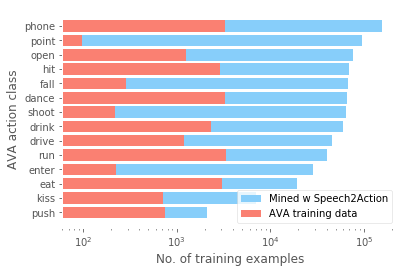
\includegraphics[width=0.9\linewidth]{images/training_dist.png}
\vspace{-0.8em}
        \end{center}
\end{minipage}
}
\headerbox{\bf\color{blue} Project Page}{name=proj,column=0,below=mining,span=2}{
More details at:  \small{\url{https://www.robots.ox.ac.uk/~vgg/research/speech2action/}}

}

\end{poster}
\end{document}
